\chapter{Auswertung und Ergebnisse}
\label{ch:auswertung-ergebnisse}

Auf Basis der theoretischen Überlegungen sowie den im vorherigen Kapitel formulierten Fragestellungen sollen nun die Hypothesen getestet werden.
Zum Erreichen dieses Ziels werden zunächst die erhobenen Daten aufbereitet, um anschließend Aussagen über die vorliegende Stichprobe treffen zu können.
Im Anschluss daran wird mithilfe statistischer Methoden analysiert, welche Informationen die gemessenen Werte liefern und welche Rückschlüsse daraus in Bezug auf die aufgestellten Hypothesen gezogen werden können.

Die Datenaufbereitung sowie deskriptive und Inferenzsstatistik wurden mithilfe der Skriptsprache R durchgeführt.
Der vollständige Code ist einsehbar in \autoref{app:r-code}.


\section{Datenaufbereitung}
\label{sec:datenaufbereitung}

Bevor die erhobenen Daten für statistische Zwecke verwendet werden können, müssen sie zunächst in Hinblick auf ihre Qualität beurteilt und mögliche Verunreinigungen der Werte korrigiert werden.
Weiterhin müssen die rohen Daten für ihre Verwendbarkeit zunächst einer Aufbereitung unterzogen werden.

Der Notwendigkeit der manuellen Bereinigung und Aufbereitung der Daten wurde bereits durch viele Einstellungen bei der Erstellung des Fragebogens entgegengewirkt.
Beispielsweise wurden die Items der Bias-Awareness-Skala, die invertiert codiert sind, bereits im Fragebogen als solche gekennzeichnet.
Dies hatte den Vorteil, dass in den exportierten Daten bereits korrekt gepolte Werte vorlagen und diese nicht erst umcodiert werden mussten.

Weiterhin wurde durch Eingabefilter verhindert, dass Werte fehlerhaft eingegeben wurden oder ganz fehlten.
Es wurde zum Beispiel jede Frage als verpflichtend gekennzeichnet, so dass erst bei Abbruch des Fragebogens fehlende Werte auftreten konnten.
In Fällen, bei denen es Sinn ergab, wurden außerdem nur korrekte Eingaben zugelassen.
Beispielsweise konnte bei der Frage nach dem Alter lediglich eine Ganzzahl zwischen 1 und 99 eingegeben werden.

Durch eine Filterfrage wurde außerdem sichergestellt, nur Studierende Fragen beantworteten, welche an diese Zielgruppe gerichtet waren.
Ebenso wurden Fragen, welche sich ausschließlich an fertig ausgebildete Lehrkräfte richteten, durch die Filterfrage nur an diese Gruppe gestellt.
Durch dieses Vorgehen musste nicht erst identifiziert werden, welche Werte überhaupt von einer Person aus der zulässigen Gruppe stammten.

Im ersten Schritt der Datenbereinigung wurden fehlerhafte Bearbeitungen des Fragebogens entfernt sowie Interviews mit unzureichenden Informationen, beispielsweise durch einen frühen Abbruch des Nutzers, gelöscht.
Zunächst wurden dabei sämtliche Interviews herausgefiltert, welche vor Beantwortung der Fragen zur Bias Awareness in Bezug auf schulischen Kontext abgebrochen wurden.
In einem zweiten Schritt wurde das Interview eines Nutzers gelöscht, welcher als Bescheibung seiner aktuellen Tätigkeit lediglich das Wort ``Hallo'' angegeben hatte.

Im Anschluss daran wurden unklare Eingaben durch Studienteilnehmer korrigiert.
Diese Korrektur geschah manuell, da es sich um individuelle Unterschiede bei den Eingaben handelte.
Es wurden beispielsweise alle Studienteilnehmer, welche sich in ihrer Tätigkeitsbeschreibung als Studierende ausgewiesen hatten, jedoch noch zusätzlich als Lehrkraft arbeiteten, als Lehramtsstudierende codiert.
Auch Personen, welche zwar als Lehrkraft arbeiteten, sich jedoch im Moment in Elternzeit befanden oder aus anderen Gründen eine andere Angabe gemacht hatten, wurden korrekt als Lehrkräfte markiert.

Ebenso wurden Personen, welche sich im Referendariat befinden, als Lehramtsstudierende markiert.
Bei der Klassifizierung von Referendaren und Referendarinnen gibt es sowohl Argumente, welche für und gegen eine solche Kategorisierung sprechen.
In diesem Fall wurde die Wahl getroffen, da insbesondere der Einfluss langjähriger Berufserfahrung auf die Bias Awareness untersucht werden sollte.
Im Fall von Berufsanfängern und -anfängerinnen liegt eine solche Erfahrung noch nicht vor, weswegen die Einteilung als Lehramtsstudierende erfolgte.

Zur Identifizierung von Interviews mit niedriger Qualität wurde berechnet, wie hoch der Anteil gleicher Antworten bei den Fragen zur Bias Awareness ist.
Im Anschluss wurden alle Interviews gelöscht, welche über einem manuell festgelegten Grenzwert von 75\% lagen.
So konnte der Verfälschung der Statistik durch Eingaben von Nutzern, welche immer die selben Antworten gaben und sich nicht mit dem Inhalt der Fragen auseinander setzten, vorgebeugt werden.

Abschließend erfolgte eine Korrektur in den Datenstrukturen der Rohdaten.
Hierbei wurden beispielsweise die Werte zum Geburtsland sowie die diesbezüglich eventuell getätigten manuellen Eingaben der Studienteilnehmer kombiniert.
Außerdem wurden für jeden Teilnehmer die Mittelwerte der in den zur Bias Awareness gemachten Angaben gebildet und in einer neuen Variablen abgespeichert.
Dies geschah für jede der verwendeten Skalen.
Die hier errechneten Werte bilden die Basis für die in \autoref{sec:inferenzstatistik} diskutierten statistischen Methoden wie Hypothesentests.


\section{Deskriptive Statistik}
\label{sec:deskriptive-statistik}

Bei der Bereinigung und Aufbereitung der Rohdaten sind bereits viele Studienteilnehmer gefiltert worden, deren Angaben fehlerhaft oder nicht verwendbar waren.
Im Folgenden kann nun die bereinigte Gruppe beschrieben und statistische Angaben über die Stichprobe gemacht werden.
Die Interviews der Studienteilnehmer wurden in Hinblick auf die Forschungsfragen und Hypothesen in zwei Gruppen geteilt.
Diesen Gruppen wurden die Teilnehmer zugeordnet in Abhängigkeit davon, ob es sich um Lehramtsstudierende bzw. Personen im Referendariat handelte oder um fertig ausgebildete Lehrkräfte.
Im Folgenden werden daher sowohl die gesamte Stichprobe sowie jede der beiden Gruppen beschrieben.

\subsection{Gesamte Stichprobe}
\label{subsec:gesamte-stichprobe}

In der Grundgesamtheit der vorliegenden Daten befanden sich N = 89 Studienteilnehmer, von denen 15\% männlich, 85\% weiblich und 0\% divers waren.
Das mittlere Alter der Studienteilnehmer betrug 31.9 Jahre (SD = 10.8).
79\% der Befragten gaben an, bereits Lehrerfahrung zu besitzen, wobei die Erfahrung im Mittel bei 6.3 Jahren lag (SD = 8.4).
Unter den Teilnehmern befanden sich 10\%, die selbst einen Migrationshintergrund hatten.
Als Migrationshintergrund wurde hierbei verstanden, dass entweder die Befragten selbst oder mindestens ein Elternteil außerhalb von Deutschland geboren wurde.

Bei Betrachtung der erlangten Abschlüsse zeigte sich ein diverses Bild.
1\% der Studienteilnehmer hatten einen Hauptschulabschluss gemacht, 12\% einen Realschulabschluss, 75\% Abitur, 28\% einen Bachelor-Abschluss, 20\% einen Master-Abschluss, 2\% Diplom, 54\% ein abgeschlossenes Staatsexamen sowie 2\% eine abgeschlossene Promotion.

\subsection{Lehramtsstudierende}
\label{subsec:lehramtsstudierende}

Unter den Studienteilnehmern befanden sich N = 35 Lehramtsstudierende, welche zu 9\% männlich, 91\% weiblich und 0\% divers waren.
Das mittlere Alter der Studierenden betrug 23.5 Jahre (SD = 2.7).
Von ihnen gaben 46\% an, bereits Lehrerfahrung zu besitzen, wobei die Erfahrung im Mittel bei 0.8 Jahren lag (SD = 1.2).
94\% der Teilnehmer gaben an, bereits das 3-wöchige Orientierungspraktikum oder das 12-wöchige Schulpraxissemester abgeschlossen zu haben.
Unter den Studierenden befanden sich 11\%, die selbst einen Migrationshintergrund hatten.

Die Studiendauer der befragten Personen lag bei 6.9 Semestern (SD = 3.9).
3\% der Studierenden hatten einen Hauptschulabschluss gemacht, 20\% einen Realschulabschluss, 77\% Abitur, 31\% einen Bachelor-Abschluss, 17\% einen Master-Abschluss sowie 14\% ein abgeschlossenes Staatsexamen. 

\subsection{Lehrkräfte}
\label{subsec:lehrkräfte}

Von den Studienteilnehmern waren N = 54 fertig ausgebildete Lehrkräfte.
19\% von diesen waren männlichen Geschlechts, 81\% weiblich und 0\% divers.
Im Mittel waren die Lehrkräfte 37.3 Jahre alt (SD = 10.7) und die durchschnittliche Lehrerfahrung betrug 9.8 Jahre (SD = 9.1).
9\% der befragten Personen hatte selbst einen Migrationshintergrund.

In Bezug auf die erlangten Abschlüsse ergaben sich folgende Informationen:
7\% der Lehrkräfte hatten einen Hauptschulabschluss gemacht, 74\% Abitur, 26\% einen Bachelor-Abschluss, 22\% einen Master-Abschluss, 4\% Diplom, 80\% ein abgeschlossenes Staatsexamen sowie 4\% eine abgeschlossene Promotion.

Von den befragten Lehrkräften waren zum Befragungszeitpunkt 13\% an einer Grundschule tätig, 39\% in der Sekundarstufe 1, 35\% am Gymnasium, 7\% an einer sonderpädagogischen Schule sowie 6\% an Gemeinschafts- und Gesamtschulen.

\subsection{Skalenkonsistenz}
\label{subsec:skalenkonsistenz}

Auf Basis der in der Studie gesammelten Daten wurde die interne Konsistenz der verwendeten Skalen überprüft.
Hierzu wurde für jede Skala Cronbach's Alpha berechnet.
Auch dabei wurden die Werte sowohl für die gesamte Stichprobe als auch in Bezug auf Lehrkräfte und Studierende berechnet.
Die Ergebnisse der Berechnungen sind in \autoref{tab:cronbachs-alpha} aufgestellt.

\begin{table}[h!]
	\begin{tabularx}{\textwidth}{X | r | r | r}
		\hline
		Variable & \textbf{$\alpha_{ges}$} & \textbf{$\alpha_{STU}$} & \textbf{$\alpha_{LK}$}\\
		\hline
		BA01: Allgemein & 0.7 & 0.64 & 0.73\\
		BA02: Allgemein -- Migrationshintergrund & 0.81 & 0.83 & 0.79\\
		BA03: Allgemein -- sozioökonomischer Hintergrund & 0.79 & 0.87 & 0.7\\
		BA04: Allgemein -- Frauen & 0.73 & 0.63 & 0.77\\
		BA05: Allgemein -- Männer & 0.8 & 0.81 & 0.79\\
		BA06: Schülerinnen und Schüler & 0.77 & 0.7 & 0.77\\
		BA07: eigene Schülerinnen und Schüler & 0.73 & 0.79 & 0.69\\
		BA08: Schülerinnen und Schüler -- Migrationshintergrund & 0.84 & 0.84 & 0.82\\
		BA09: Schülerinnen und Schüler -- sozioökonomischer Hintergrund & 0.82 & 0.81 & 0.82\\
		BA10: Schülerinnen und Schüler -- Frauen & 0.73 & 0.79 & 0.68\\
		BA11: Schülerinnen und Schüler -- Männer & 0.8 & 0.8 & 0.8\\
		\hline
	\end{tabularx}
	\caption{Cronbach's Alpha (raw) der verschiedenen Bias Awareness Skalen bei unterschiedlichen Stichproben}
	\label{tab:cronbachs-alpha}
\end{table}


\section{Inferenzstatistik}
\label{sec:inferenzstatistik}

Im Folgenden sollen mithilfe der erhobenen Daten Rückschlüsse von der Stichprobe auf die Allgemeinheit gezogen werden.
Im Fokus steht hierbei die Überprüfung der in \autoref{sec:hypothesen} formulierten Hypothesen.
Hierzu wurden zunächst die Mittelwerte der verschiedenen Skalen berechnet und anschließend miteinander verglichen.
Um zu untersuchen, ob es sich bei den Differenzen um statistisch signifikante Abweichungen handelt, wurden abhängige t-Tests verwendet.
Die Entscheidung für einen abhängigen Test beruhte dabei auf der Tatsache, dass es sich in allen getesteten Fällen um die Messwerte zwei verschiedener Skalen bei derselben Testperson handelt.

\subsection{Überprüfung der Verteilungen}
\label{subsec:normalverteilung}

Eine notwendige Voraussetzung für das Anwenden eines t-Tests ist die Normalverteilung der Variable.
Bevor die Tests durchgeführt werden können muss also zunächst überprüft werden, ob diese Bedingung erfüllt ist.
Hierfür wurde für den Mittelwert jeder Skala ein Shapiro-Wilk-Test durchgeführt.
Das Signifikanzniveau wurde dabei auf $\alpha=0.05$ festgelegt.
Der Shapiro-Wilk-Test wurde sowohl für die gesamte Stichprobe, als auch für die Teilgruppe der Lehrkräfte und der Lehramtsstudierenden angewendet.
Die Ergebnisse des Tests sind in \autoref{tab:shapiro-wilk} dargestellt.

\begin{table}[h!]
	\begin{tabularx}{\textwidth}{X | r | r | r}
		\hline
		Variable & $p_{ges}$ & $p_{STU}$ & $p_{LK}$ \\
		\hline
		BA01: Allgemein & 0.41 & 0.19 & 0.33\\
		BA02: Allgemein -- Migrationshintergrund & 0.18 & 0.02 & 0.62\\
		BA02: Allgemein -- sozioökonomischer Hintergrund & 0.31 & 0.56 & 0.31\\
		BA03: Allgemein -- Frauen & <0.001 & <0.001 & <0.001\\
		BA04: Allgemein -- Männer & <0.001 & 0.10 & 0.01\\
		BA05: Schülerinnen und Schüler & 0.26 & 0.49 & 0.56\\
		BA06: eigene Schülerinnen und Schüler & 0.19 & 0.23 & 0.04\\
		BA07: Schülerinnen und Schüler -- Migrationshintergrund & 0.10 & 0.12 & 0.45\\
		BA08: Schülerinnen und Schüler -- sozioökonomischer Hintergrund & 0.20 & 0.11 & 0.21\\
		BA09: Schülerinnen und Schüler -- Frauen & <0.001 & <0.001 & <0.001\\
		BA10: Schülerinnen und Schüler -- Männer & <0.001 & 0.02 & 0.02\\
		\hline
	\end{tabularx}
	\caption{Ergebnisse des Shapiro-Wilk-Tests der Mittelwerte der verschiedenen Bias Awareness Skalen bei unterschiedlichen Stichproben}
	\label{tab:shapiro-wilk}
\end{table}

Es ergab sich, dass zahlreiche Werte unter dem festgelegten Signifikanzniveau von 0.05 liegen.
Eine Untersuchung der Histogramme zeigte, dass es sich möglicherweise um Variablen mit einer verschobenen und zusätzlich abgeschnittenen Normalverteilung handeln könnte.
Da der t-Test in gewissem Maße robust gegenüber abgeschnittenen Normalverteilungen ist, wurde dieser nachfolgend trotzdem angewendet.
Dennoch wurde zusätzlich bei den betroffenen Variablen auch ein Wilcoxon-Vorzeichen-Rang-Test für abhängige Stichproben verwendet, welcher auch bei nicht-normalverteilten Variablen genutzt werden kann.

\subsection{Ergebnisse zur gesamten Stichprobe}
\label{subsec:ergebnisse-gesamt}

Zur Überprüfung der Hypothesen H1 und H2 wurden die Differenzen zwischen den Mittelwerten der allgemeinen Bias Awareness Skala (BA01), der allgemeinen Skala mit schulspezifisch formulierten Items (BA06) sowie der Skala mit Bezug auf eigene Schülerinnen und Schüler (BA07) untersucht.
Die Ergebnisse dieser Untersuchung sind in \autoref{fig:boxplot-allgemein-gesamt} dargestellt.

\begin{figure}[h!]
	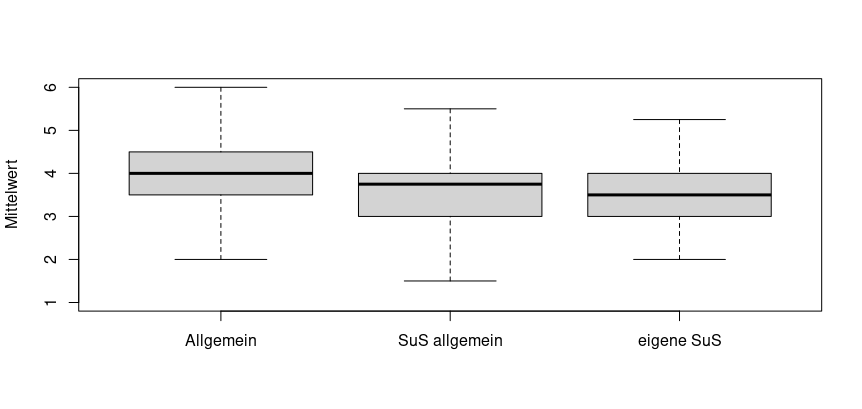
\includegraphics[width=\textwidth]{resources/boxplot-allgemein-gesamt.png}
	\caption{Unterschiede in den Mittelwerten bei Erfassung mit allgemeiner vs. schulspezifischer Skala}
	\label{fig:boxplot-allgemein-gesamt}
\end{figure}

Um die statistische Relevanz der berechneten Differenzen in den Mittelwerten zu überprüfen, wurden jeweils zweiseitige abhängige t-Tests angewendet.
Die Ergebnisse dieser Tests sind in \autoref{tab:t-tests-allgemein-gesamt} zusammengefasst.

\begin{table}[h!]
	\begin{tabularx}{\textwidth}{X | r | r | r | r | r | r}
		\hline
		Variable & M & SD & df & t & p & Cohen's d\\
		\hline
		BA01 - BA06 & 0.463 & 0.896 & 87 & 4.849 & <0.001 & 0.517\\
		BA01 - BA07 & 0.546 & 0.881 & 86 & 5.778 & <0.001 & 0.619\\
		BA06 - BA07 & 0.075 & 0.541 & 86 & 1.289 & 0.201 & 0.138\\
		\hline
	\end{tabularx}
	\caption{Ergebnisse der zweiseitigen abhängigen t-Tests bei Vergleich allgemeiner und schulspezifischer Formulierung}
	\label{tab:t-tests-allgemein-gesamt}
\end{table}

Die mit der allgemeinen Skala gemessene Bias Awareness (M = 4.03, SD = 0.85) war signifikant höher als die mit der auf Schülerinnen und Schüler formulierten Skala erhobene Bias Awareness (M = 3.56, SD = 0.88); mit t(88) = 4.849; p < 0.001; d = 0.517.
Nach \citet{cohen1992power} handelt es sich somit um einen mittleren Effekt.

Bei Messung mit der allgemeinen Skala (M = 4.03, SD = 0.85) war die gemessene Bias Awareness ebenfalls signifikant höher als bei Messung mit in Bezug auf selbst unterrichtete Schülerinnen und Schüler formulierter Skala (M = 3.49, SD = 0.81); mit t(88) = 5.778; p < 0.001; d = 0.619.
Auch hier handelt es sich um einen mittleren Effekt \citep{cohen1992power}.

Die Differenz zwischen der Messung mit der auf Schülerinnen und Schüler bezogenen Skala (M = 3.56, SD = 0.88) und der in Bezug auf selbst unterrichtete Schülerinnen und Schüler formulierten Skala (M = 3.49, SD = 0.81) war nicht signifikant; mit t(88) = 1.289; p = 0.201; d = 0.138.

Um Hypothese 3 zu testen wurden jeweils die Mittelwerte der Skalen mit stereotypenspezifischer Formulierung gebildet und mit den Mittelwerten der Skalen mit schul- und stereotypenspezifischer Formulierung verglichen.
Eine Übersicht über die gemessenen Werte sind in \autoref{fig:boxplot-stereotypen-gesamt} abgebildet.

\begin{figure}[h!]
	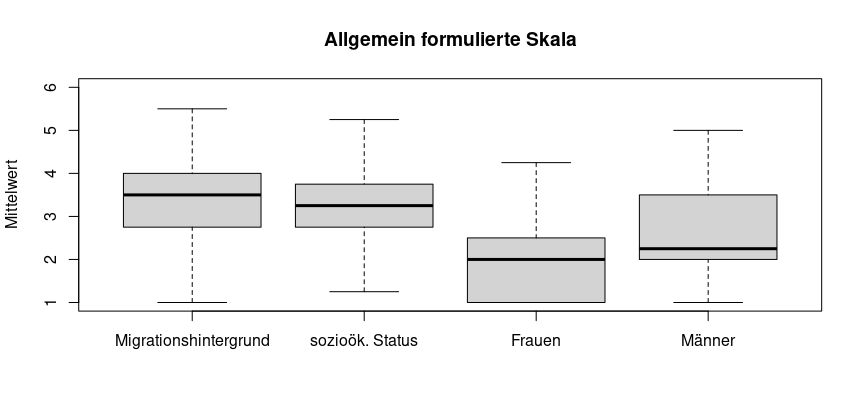
\includegraphics[width=\textwidth]{resources/boxplot-stereotypen-1-gesamt.png}
	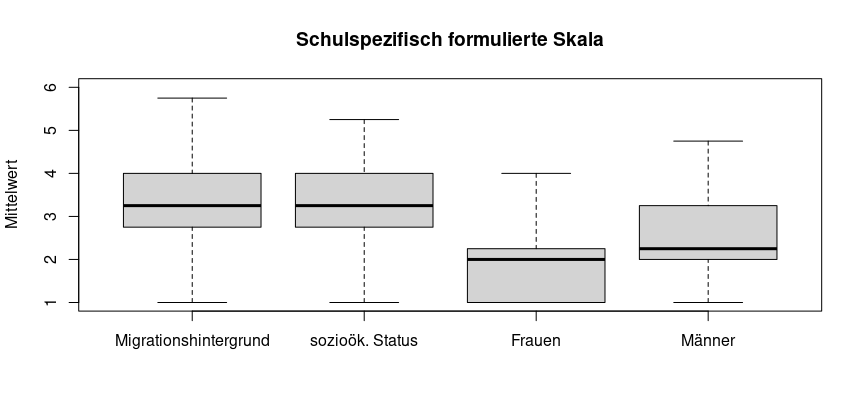
\includegraphics[width=\textwidth]{resources/boxplot-stereotypen-2-gesamt.png}
	\caption{Unterschiede in den Mittelwerten bei Erfassung der stereotypenspezifischen Bias Awareness mit allgemeiner vs. schulspezifischer Skala}
	\label{fig:boxplot-stereotypen-gesamt}
\end{figure}

Verglichen wurden jeweils die allgemeinen Skalen zu Migrationshintergrund (BA02), sozioökonomischem Status (BA03) sowie in Bezug auf Frauen (BA04) und Männer (BA05) mit den schulspezifisch formulierten Skalen zu Migrationshintergrund (BA08), sozioökonomischem Status (BA09), Frauen (BA10) und Männern (BA11).
Um zu überprüfen, ob es sich bei den Abweichungen um statistisch signifikante Differenzen handelt, wurden erneut zweiseitige abhängige t-Tests verwendet.
Die Effektstärke wurde mithilfe von Cohen's d angegeben.
Da keine der geschlechtsbezogenen Skalen den Shapiro-Wilk-Test bestanden hatte, wurde in diesen Fällen zusätzlich ein Wilcoxon-Test durchgeführt und die Wilcoxon-Effektstärke r berechnet.
Die Ergebnisse sind in \autoref{tab:t-tests-stereotypen-gesamt} dargestellt.

\begin{table}[h!]
	\begin{tabularx}{\textwidth}{X | r | r | r | r | r | r}
		\hline
		Variable & M & SD & df & t & p & Cohen's d\\
		\hline
		BA02 - BA08 & 0.107 & 0.613 & 83 & 1.603 & 0.113 & 0.175\\
		BA03 - BA09 & 0.158 & 0.577 & 83 & 2.507 & 0.014 & 0.274\\
		BA04 - BA10 (t-Test) & 0.077 & 0.618 & 80 & 1.123 & 0.265 & 0.125\\
		BA04 - BA10 (Wilcoxon-Test) & & & & & 0.254 & r = 0.23\\
		BA05 - BA11 (t-Test) & 0.133 & 0.775 & 80 & 1.542 & 0.127 & 0.171\\
		BA05 - BA11 (Wilcoxon-Test) & & & & & 0.369 & r = 0.15\\
		\hline
	\end{tabularx}
	\caption{Ergebnisse der zweiseitigen abhängigen t-Tests bzw. Wilcoxon-Vorzeichen-Rang-Tests bei Erfassung der stereotypenspezifischen Bias Awareness mit allgemeiner vs. schulspezifischer Skala}
	\label{tab:t-tests-stereotypen-gesamt}
\end{table}

Signifikante Effekte zeigten sich lediglich beim Vergleich der allgemeinen, in Bezug auf sozioökonomischen Status formulierten Skala (M = 3.37, SD = 0.88) und ihrer schulspezifischen Variante (M = 3.23, SD = 0.9); mit t(83) = 2.507; p = 0.014; d = 0.274.
Hierbei handelt es sich allerdings nur um einen schwachen Effekt.

Bei allen anderen getesteten Variablen konnte keine statistische Signifikanz festgestellt werden.
Auch die Verwendung des Wilcoxon-Vorzeichen-Rang-Tests in Fällen, in denen der Shapiro-Wilk-Test fehlgeschlagen war, lieferte keinen Hinweis auf statistisch signifikante Abweichungen.

\subsection{Ergebnisse zu Lehramtsstudierenden}
\label{subsec:ergebnisse-studierende}

Nachdem in \autoref{subsec:ergebnisse-gesamt} Aussagen zur gesamten Stichprobe getroffen wurden, werden im Folgenden nur die erhobenen Daten von Lehramtsstudierenden betrachtet.
Dabei werden erneut zuerst die Differenzen zwischen den Skalen zur allgemeinen Bias Awareness (BA01) betrachtet, jeweils generell sowie in Bezug auf Schülerinnen und Schüler (BA06) sowie selbst unterrichtete Schülerinnen und Schüler (BA07).
Die Ergebnisse bei Einschränkung auf die Gruppe der Lehramtsstudierenden finden sich hierbei in \autoref{fig:boxplot-allgemein-studierende}.

\begin{figure}[h!]
	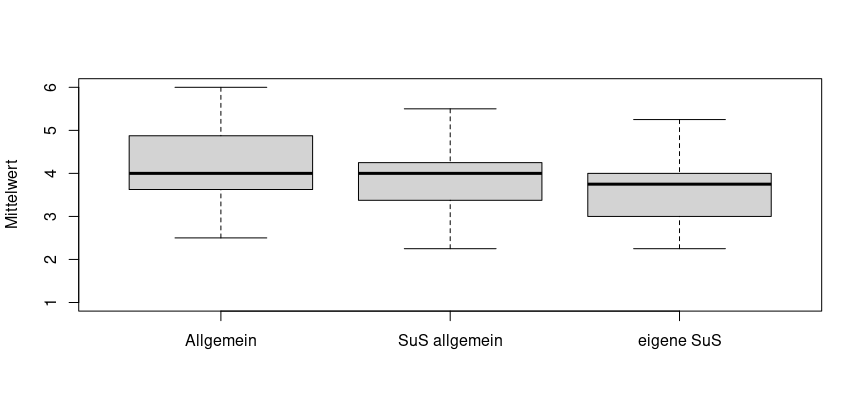
\includegraphics[width=\textwidth]{resources/boxplot-allgemein-studierende.png}
	\caption{Unterschiede in den Mittelwerten bei Erfassung mit allgemeiner vs. schulspezifischer Skala, eingeschränkt auf Lehramtsstudierende}
	\label{fig:boxplot-allgemein-studierende}
\end{figure}

Die statistische Relevanz der Differenzen wurde mithilfe eines zweiseitigen abhängigen t-Tests geprüft.
Aufgestellt sind die Ergebnisse dieser Tests in \autoref{tab:t-tests-allgemein-studierende}.

\begin{table}[h!]
	\begin{tabularx}{\textwidth}{X | r | r | r | r | r | r}
		\hline
		Variable & M & SD & df & t & p & Cohen's d\\
		\hline
		BA01 - BA06 & 0.336 & 0.998 & 34 & 1.99 & 0.055 & 0.336\\
		BA01 - BA07 & 0.640 & 1.048 & 33 & 3.558 & 0.001 & 0.610\\
		BA06 - BA07 & 0.287 & 0.530 & 33 & 3.156 & 0.003 & 0.541\\
		\hline
	\end{tabularx}
	\caption{Ergebnisse der zweiseitigen abhängigen t-Tests bei Vergleich allgemeiner und schulspezifischer Formulierung, eingeschränkt auf Lehramtsstudierende}
	\label{tab:t-tests-allgemein-studierende}
\end{table}

Für die allgemein formulierte Skala zur Messung der Bias Awareness (M = 4.2, SD = 0.87) im Vergleich mit der auf Schülerinnen und Schüler bezogenen Skala (M = 3.86, SD = 0.81) konnte keine statistische Signifikanz gemessen werden (p = 0.055 > 0.05 = $\alpha$).

Zwischen der allgemeinen Skala (M = 4.2, SD = 0.87) und der auf selbst unterrichtete Schülerinnen und Schüler bezogenen Skala (M = 3.59, SD = 0.85) bestand ein signifikanter Unterschied; mit t(33) = 3.558; p = 0.001; d = 0.61.
Nach \citep{cohen1992power} stellt die gemessene Differenz einen Effekt mittlerer Stärke dar.

Weiterhin konnte ein statistisch signifikanter Unterschied zwischen der allgemein schulbezogenen Skala (M = 3.86, SD = 0.81) und der auf eigene Schülerinnen und Schüler formulierten Skala (M = 3.59, SD = 0.85) festgestellt werden; mit t(33) = 3.156; p = 0.003; d = 0.541.
Auch hier handelt es sich um einen mittleren Effekt.

\begin{figure}[h!]
	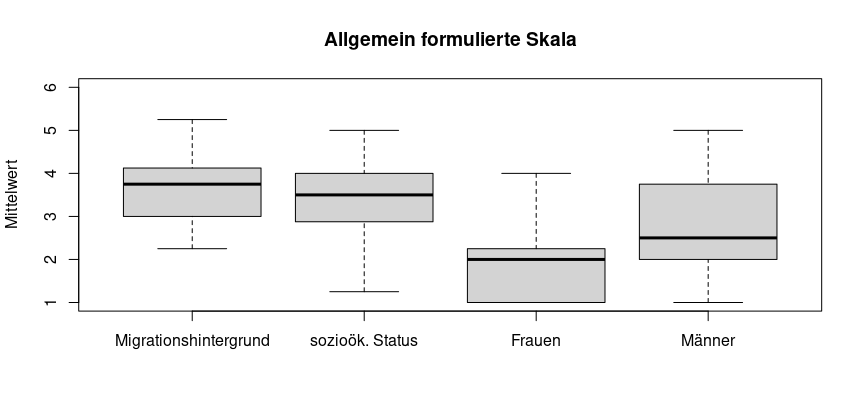
\includegraphics[width=\textwidth]{resources/boxplot-stereotypen-1-studierende.png}
	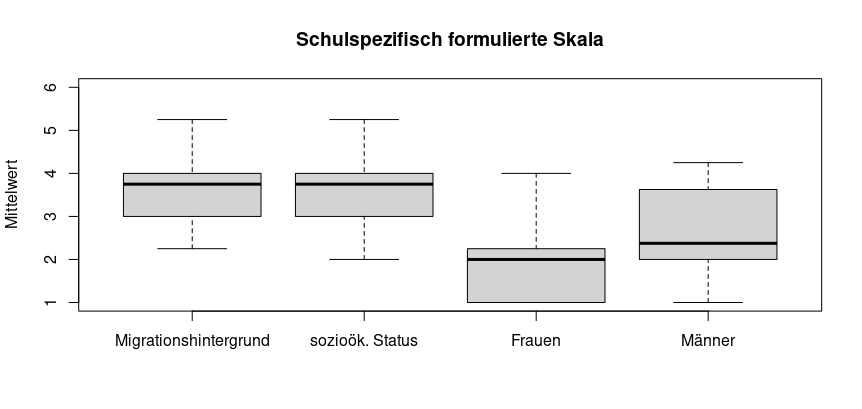
\includegraphics[width=\textwidth]{resources/boxplot-stereotypen-2-studierende.png}
	\caption{Unterschiede in den Mittelwerten bei Erfassung der stereotypenspezifischen Bias Awareness mit allgemeiner vs. schulspezifischer Skala, eingeschränkt auf Lehramtsstudierende}
	\label{fig:boxplot-stereotypen-studierende}
\end{figure}

Ebenso wurden die Mittelwerte der stereotypenspezifisch formulierten Skala zur Messung der Bias Awareness mit der schul- und stereotypenspezifisch formulierten Skala verglichen.
Die Ergebnisse\break sind in \autoref{fig:boxplot-stereotypen-studierende} dargestellt.

Auch hier wurden jeweils die allgemeinen Skalen zu Migrationshintergrund (BA02), sozioökonomischem Status (BA03), in Bezug auf Frauen (BA04) und in Bezug auf Männer (BA05) mit den jeweiligen schulspezifisch formulierten Skalen zu Migrationshintergrund (BA08), sozioökonomischem Status (BA09), Frauen (BA10) und Männern (BA11) verglichen.
Für die Überprüfung der statistischen Signifikanz wurden zweiseitige abhängige t-Tests verwendet.
Die Effektstärken wurden mithilfe Cohen's d berechnet.
In den Fällen, in welchen der Shapiro-Wilk-Test fehlgeschlagen war, wurde zusätzlich zum t-Test ein Wilcoxon-Vorzeichen-Rang-Test verwendet sowie die Wilcoxon-Effektstärke r berechnet.
Die Ergebnisse der Tests sind in \autoref{tab:t-tests-stereotypen-studierende} aufgelistet.

\begin{table}[h!]
	\begin{tabularx}{\textwidth}{X | r | r | r | r | r | r}
		\hline
		Variable & M & SD & df & t & p & Cohen's d\\
		\hline
		BA02 - BA08 (t-Test) & -0.015 & 0.649 & 32 & -0.134 & 0.894 & 0.023\\
		BA02 - BA08 (Wilcoxon-Test) & & & & & 0.961 & r = -0.01\\
		BA03 - BA09 & 0.008 & 0.666 & 32 & 0.065 & 0.948 & 0.011\\
		BA04 - BA10 (t-Test) & -0.086 & 0.498 & 31 & -0.975 & 0.337 & 0.172\\
		BA04 - BA10 (Wilcoxon-Test) & & & & & 0.430 & r = -0.27\\
		BA05 - BA11 (t-Test) & 0.086 & 0.548 & 31 & 0.886 & 0.382 & 0.157\\
		BA05 - BA11 (Wilcoxon-Test) & & & & & 0.404 & r = 0.23\\
		\hline
	\end{tabularx}
	\caption{Ergebnisse der zweiseitigen abhängigen t-Tests bzw. Wilcoxon-Vorzeichen-Rang-Tests bei Erfassung der stereotypenspezifischen Bias Awareness mit allgemeiner vs. schulspezifischer Skala, eingeschränkt auf Lehramtsstudierende}
	\label{tab:t-tests-stereotypen-studierende}
\end{table}

Bei keiner der getesteten Variablen konnte ein statistisch signifikanter Unterschied festgestellt werden.
Auch in den Fällen, in denen nicht-normalverteilte Variablen getestet wurden konnte der zusätzlich durchgeführte Wilcoxon-Vorzeichen-Rang-Test keine statistische Signifikanz feststellen.

\subsection{Ergebnisse zu Lehrkräften mit Praxiserfahrung}
\label{subsec:ergebnisse-lehrkraefte}

Analog zum Vorgehen in \autoref{subsec:ergebnisse-studierende} wurde ebenfalls die Gruppe der Lehrkräfte in der vorliegenden Stichprobe einzeln betrachtet.
Auch hier wurden zunächst die Differenzen zwischen der allgemeinen Skala zur Bias Awareness (BA01) und den Skalen mit Formulierungen mit Bezug auf Schülerinnen und Schüler (BA06) sowie eigene Schülerinnen und Schüler (BA07) untersucht.
Die Ergebnisse des lehrkraftbezogenen Vergleichs sind in \autoref{fig:boxplot-allgemein-lehrkraefte} dargestellt.

\begin{figure}[h!]
	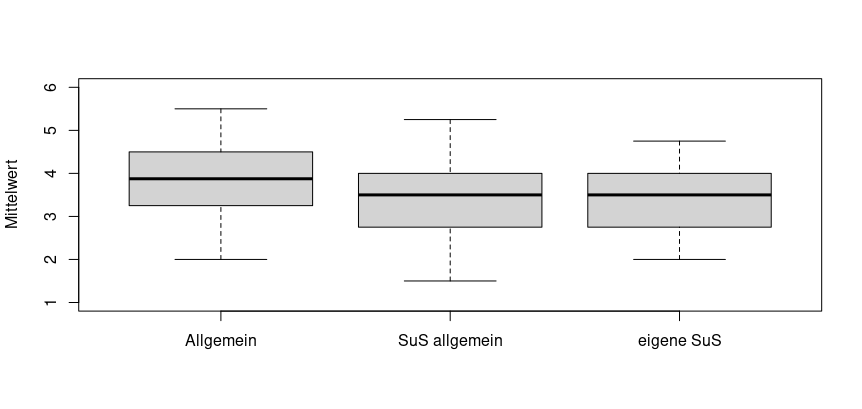
\includegraphics[width=\textwidth]{resources/boxplot-allgemein-lehrkraefte.png}
	\caption{Unterschiede in den Mittelwerten bei Erfassung mit allgemeiner vs. schulspezifischer Skala, eingeschränkt auf Lehrkräfte mit Praxiserfahrung}
	\label{fig:boxplot-allgemein-lehrkraefte}
\end{figure}

Zur Überprüfung der statistischen Relevanz wurden zweiseitige abhängige t-Tests angewandt.
Die Effektstärke wurde durch Cohen's d berechnet.
Da der Shapiro-Wilk-Test bei der auf selbst unterrichtete Schülerinnen und Schüler bezogenen Skala (BA07) fehlgeschlagen war, wurde hier zusätzlich ein Wilcoxon-Vorzeichen-Rang-Test durchgeführt sowie die Wilcoxon-Effektstärke r angegeben.
Die Ergebnisse der durchgeführten Tests sind in \autoref{tab:t-tests-allgemein-lehrkraefte} aufgestellt.

\begin{table}[h!]
	\begin{tabularx}{\textwidth}{X | r | r | r | r | r | r}
		\hline
		Variable & M & SD & df & t & p & Cohen's d\\
		\hline
		BA01 - BA06 & 0.547 & 0.820 & 52 & 4.855 & <0.001 & 0.667\\
		BA01 - BA07 (t-Test) & 0.486 & 0.760 & 52 & 4.653 & <0.001 & 0.639\\
		BA01 - BA07 (Wilcoxon-Test) & & & & & <0.001 & r = 0.69\\
		BA06 - BA07 (t-Test) & -0.061 & 0.507 & 52 & -0.881 & 0.383 & 0.123\\
		BA06 - BA07 (Wilcoxon-Test) & & & & & 0.481 & r = -0.13\\
		\hline
	\end{tabularx}
	\caption{Ergebnisse der zweiseitigen abhängigen t-Tests bei Vergleich allgemeiner und schulspezifischer Formulierung, eingeschränkt auf Lehrkräfte mit Praxiserfahrung}
	\label{tab:t-tests-allgemein-lehrkraefte}
\end{table}

Die Differenz der Mittelwerte bei Messung der Bias Awareness mit allgemeiner Skala (M = 3.92, SD = 0.82) im Vergleich zur Messung mit auf Schülerinnen und Schüler bezogener Skala (M = 3.36, SD = 0.87) stellte einen statistisch signifikanten Unterschied dar; mit t(52) = 4.855; p < 0.001; d = 0.667.
Nach \citet{cohen1992power} handelt es sich dabei um einen Effekt mittlerer Stärke.

Auch die Unterschiede bei Messung mit der allgemeinen Skala (M = 3.92, SD = 0.82) verglichen mit der auf selbst unterrichtete Schülerinnen und Schüler formulierten Skala (M = 3.42, SD = 0.78) waren statistisch signifikant; mit t(52) = 4.653; p < 0.001; d = 0.639.
Der zusätzlich durchgeführte Wilcoxon-Test bestätigte dies; mit p < 0.001; r = 0.69.
Auch hier handelt es sich um einen mittleren Effekt.

Bei Vergleich der in Bezug auf Schülerinnen und Schüler formulierten Skala (M = 3.36, SD = 0.87) und der in Bezug auf selbst unterrichtete Schülerinnen und Schüler formulierten Skala (M = 3.42, SD = 0.78) konnte weder mit dem t-Test (t(52) = -0.881; p = 0.383; d = 0.123) noch mit dem Wilcoxon-Test (p = 0.481; r = -0.13) statistische Signifikanz festgestellt werden.

Zusätzlich zum Vergleich der allgemeinen Skalen wurden auch die allgemein formulierten stereotypenspezifischen Skalen jeweils mit ihrer schulspezifisch formulierten Variante verglichen.
Die Ergebnisse bei Betrachtung von Lehrkräften mit Praxiserfahrung sind in \autoref{fig:boxplot-stereotypen-lehrkraefte} dargestellt.

\begin{figure}[h!]
	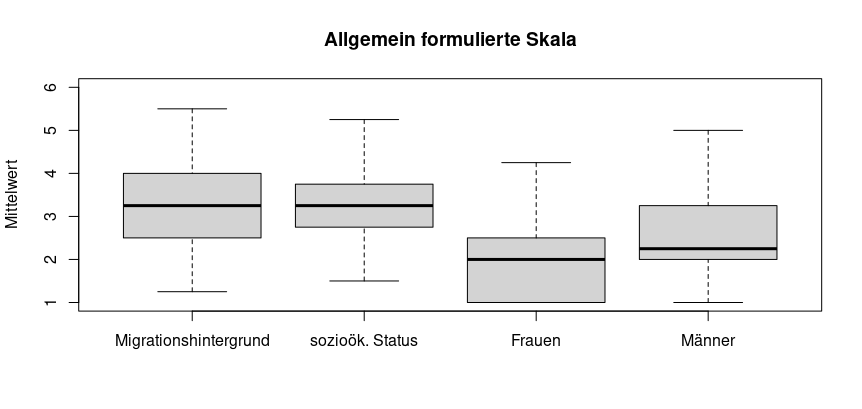
\includegraphics[width=\textwidth]{resources/boxplot-stereotypen-1-lehrkraefte.png}
	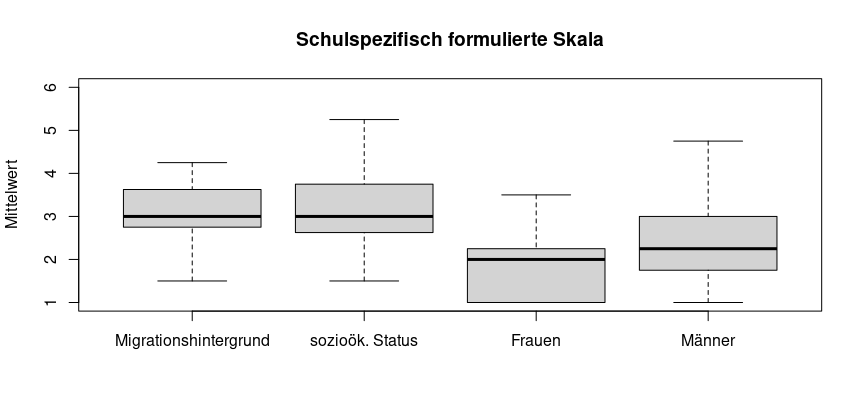
\includegraphics[width=\textwidth]{resources/boxplot-stereotypen-2-lehrkraefte.png}
	\caption{Unterschiede in den Mittelwerten bei Erfassung der stereotypenspezifischen Bias Awareness mit allgemeiner vs. schulspezifischer Skala, eingeschränkt auf Lehrkräfte mit Praxiserfahrung}
	\label{fig:boxplot-stereotypen-lehrkraefte}
\end{figure}

Wie auch beim Vergleich der allgemeinen Skalen wurden zur Überprüfung der statistischen Signifikanz zweiseitige abhängige t-Tests durchgeführt und die Effektstärken in Form von Cohen's d berechnet.
In den Fällen, in denen der Shapiro-Wilk-Test negativ ausgefallen war, wurde zusätzlich ein Wilcoxon-Vorzeichen-Rang-Test durchgeführt und die zugehörige Effektstärke r angegeben.
Die Ergebnisse der Tests sind in \autoref{tab:t-tests-stereotypen-lehrkraefte} aufgelistet.

\begin{table}[h!]
	\begin{tabularx}{\textwidth}{X | r | r | r | r | r | r}
		\hline
		Variable & M & SD & df & t & p & Cohen's d\\
		\hline
		BA02 - BA08 & 0.186 & 0.581 & 50 & 2.291 & 0.026 & 0.321\\
		BA03 - BA09 & 0.255 & 0.762 & 50 & 3.687 & <0.001 & 0.516\\
		BA04 - BA10 (t-Test) & 0.184 & 0.669 & 48 & 1.922 & 0.061 & 0.275\\
		BA04 - BA10 (Wilcoxon-Test) & & & & & 0.046 & r = 0.50\\
		BA05 - BA11 (t-Test) & 0.163 & 0.896 & 48 & 1.275 & 0.209 & 0.182\\
		BA05 - BA11 (Wilcoxon-Test) & & & & & 0.617 & r = 0.11\\
		\hline
	\end{tabularx}
	\caption{Ergebnisse der zweiseitigen abhängigen t-Tests bzw. Wilcoxon-Vorzeichen-Rang-Tests bei Erfassung der stereotypenspezifischen Bias Awareness mit allgemeiner vs. schulspezifischer Skala, eingeschränkt auf Lehrkräfte mit Praxiserfahrung}
	\label{tab:t-tests-stereotypen-lehrkraefte}
\end{table}

Es zeigte sich, dass ein statistisch signifikanter Unterschied zwischen der allgemein formulierten Skala zu Migrationshintergrund (M = 3.29, SD = 0.93) und ihrer schulbezogenen Variante (M = 3.11, SD = 0.92) vorlag; mit t(50) = 2.291; p = 0.026; d = 0.321.
Es handelt sich hierbei um einen schwachen Effekt \citep{cohen1992power}.

Ebenso konnte statistische Signifikanz zwischen der allgemein formulierten Skala zum sozioökonomischen Status (M = 3.34, SD = 0.77) und ihrer schulbezogenen Variante (M = 3.12, SD = 0.83) festgestellt werden; mit t(50) = 3.687; p < 0.001; d = 0.516.
Es handelt sich um einen Effekt mittlerer Stärke.

Die Differenz der Mittelwerte zwischen der allgemein formulierten Skala bezogen auf Frauen (M = 2.02, SD = 1) und ihrer schulbezogenen Variante (M = 1.83, SD = 0.84) war bei Verwendung des t-Tests nicht signifikant (p = 0.061).
Der Wilcoxon-Vorzeichen-Rang-Test konnte allerdings mit p = 0.046 statistische Signifikanz bei einer Effektstärke von r = 0.50 zeigen.

Keine statistische Signifikanz konnte bei Vergleich der allgemein formulierten Skala mit Bezug auf Männer (M = 2.53, SD = 1.07) und ihre schulbezogenen Variante (M = 2.36, SD = 0.99) festgestellt werden.
Sowohl der t-Test (p = 0.209) als auch der Wilcoxon-Test (p = 0.617) lieferten ein negatives Ergebnis.


\subsection{Differenzen zwischen Lehramtsstudierenden und Lehrkräften}
\label{subsec:differenzen-studierende-lehrkraefte}

Nachdem die Ergebnisse zu den einzelnen Gruppen innerhalb der Stichprobe beschrieben wurden, kann nun untersucht werden, welche Differenzen zwischen Lehramtsstudierenden und Lehrkräften vorliegen.
Hierzu wurden pro verwendeter Skala die erreichten Mittelwerte miteinander verglichen.
Um die statistische Signifikanz der Unterschiede zu untersuchen, wurden zweiseitige Welch-t-Tests für unabhängige Stichproben verwendet.
Die Ergebnisse sind in \autoref{tab:t-tests-studierende-lehrkraefte} dargestellt.

\begin{table}[h!]
	\begin{tabularx}{\textwidth}{X | r | r | r | r | r | r}
		\hline
		Variable & M & SD (pooled) & df & t & p & Cohen's d\\
		\hline
		$BA01_{STU} - BA01_{LK}$ & 0.283 & 0.841 & 70.156 & 1.537 & 0.129 & 0.337\\
		$BA02_{STU} - BA02_{LK}$ & 0.201 & 1.002 & 64.169 & 0.893 & 0.375 & 0.201\\
		$BA03_{STU} - BA03_{LK}$ & 0.070 & 0.883 & 58.472 & 0.340 & 0.735 & 0.078\\
		$BA04_{STU} - BA04_{LK}$ & -0.195 & 0.925 & 76.187 & -0.975 & 0.333 & 0.211\\
		$BA05_{STU} - BA05_{LK}$ & 0.178 & 1.085 & 65.05 & 0.716 & 0.477 & 0.164\\
		$BA06_{STU} - BA06_{LK}$ & 0.501 & 0.847 & 76.994 & 2.761 & 0.007 & 0.591\\
		$BA07_{STU} - BA07_{LK}$ & 0.164 & 0.810 & 66.049 & 0.902 & 0.370 & 0.202\\
		$BA08_{STU} - BA08_{LK}$ & 0.438 & 1.004 & 59.164 & 1.874 & 0.066 & 0.436\\
		$BA09_{STU} - BA09_{LK}$ & 0.291 & 0.894 & 59.808 & 1.405 & 0.165 & 0.326\\
		$BA10_{STU} - BA10_{LK}$ & 0.075 & 0.873 & 62.119 & 0.369 & 0.713 & 0.086\\
		$BA11_{STU} - BA11_{LK}$ & 0.255 & 1.027 & 61.801 & 1.070 & 0.289 & 0.248\\
		\hline
	\end{tabularx}
	\caption{Ergebnisse der zweiseitigen Welch-t-Tests für unabhängige Stichproben beim Vergleich von Lehramtsstudierenden und Lehrkräften}
	\label{tab:t-tests-studierende-lehrkraefte}
\end{table}

Eine statistisch signifikante Differenz konnte lediglich beim Vergleich der Mittelwerte bei der allgemein formulierten, auf Schülerinnen und Schüler bezogenen Skala von Lehramtsstudierenden (M = 3.864, SD = 0.805) und den Lehrkräften mit Praxiserfahrung (M = 3.363, SD = 0.874) festgestellt werden; mit t(76.994) = 2.761; p = 0.007; d = 0.591.
Hierbei handelt es sich nach \citet{cohen1992power} um einen mittleren Effekt.